\documentclass[portrait]{baposter}

\usepackage{times}
\usepackage{calc}
\usepackage{graphicx}
\usepackage{amsmath}
\usepackage{amssymb}
\usepackage{relsize}
\usepackage{multirow}
\usepackage{bm}
\usepackage{psfrag}

% Mathy help
\newcommand{\parens}[1]{\!\left(#1\right)}

%% PSO Stuff
\DeclareMathOperator{\URand}{U}
\DeclareMathOperator*{\argmin}{arg\;min}
\DeclareMathOperator*{\argmax}{arg\;max}
\DeclareMathOperator*{\arginf}{arg\;inf}
\DeclareMathOperator*{\argsup}{arg\;sup}
\providecommand{\pers}{\ensuremath{P}}
\providecommand{\neigh}{\ensuremath{N}}
\providecommand{\leftind}{\ensuremath{L}}
\providecommand{\rightind}{\ensuremath{R}}
\providecommand{\nURand}{\ensuremath{U^\neigh}}
\providecommand{\pURand}{\ensuremath{U^\pers}}
\providecommand{\ppos}{\ensuremath{\Vec{x}}}
\providecommand{\pposbold}{\ensuremath{\Vec{\mathbf{x}}}}
\providecommand{\fppos}{\ensuremath{\Vec{fx}}}
\providecommand{\pvel}{\ensuremath{\Vec{v}}}
\providecommand{\nbest}{\ensuremath{\Vec{x}^\neigh}}
\providecommand{\nbestbold}{\ensuremath{\Vec{\mathbf{x}}^\mathbf{\neigh}}}
\providecommand{\fnbest}{\ensuremath{\Vec{fx}^\neigh}}
\providecommand{\pbest}{\ensuremath{\Vec{x}^\pers}}
\providecommand{\pbestbold}{\ensuremath{\Vec{\mathbf{x}}^\mathbf{\pers}}}
\providecommand{\fpbest}{\ensuremath{\Vec{fx}^\pers}}
\providecommand{\constriction}{\ensuremath{\chi}}
\providecommand{\ncoeff}{\ensuremath{\phi^\neigh}}
\providecommand{\pcoeff}{\ensuremath{\phi^\pers}}
\providecommand{\obs}{\ensuremath{\Vec{\xi}}}
\providecommand{\ofunc}{\ensuremath{f}}
\providecommand{\swarm}{\ensuremath{swarm}}

%SpecExPSO Stuff
\providecommand{\indic}{\ensuremath{I}}
\providecommand{\specvel}{\ensuremath{\vec{V}}}
\providecommand{\specpos}{\ensuremath{\vec{X}}}
\providecommand{\leftn}{\ensuremath{\Vec{x}^\leftind}}
\providecommand{\leftnbold}{\ensuremath{\Vec{\mathbf{x}}^\mathbf{\leftind}}}
\providecommand{\rightn}{\ensuremath{\Vec{x}^\rightind}}
\providecommand{\rightnbold}{\ensuremath{\Vec{\mathbf{x}}^\mathbf{\rightind}}}
\providecommand{\caseset}{\ensuremath{\mathcal{C}}}
\providecommand{\casegen}{\ensuremath{c}}
\providecommand{\casedef}{\ensuremath{(\pbest,\nbest)}}
\providecommand{\casexn}{\ensuremath{(S,-)}}
\providecommand{\casexx}{\ensuremath{(S,S)}}
\providecommand{\casexl}{\ensuremath{(S,\leftind)}}
\providecommand{\casexr}{\ensuremath{(S,\rightind)}}
\providecommand{\casepn}{\ensuremath{(-,-)}}
\providecommand{\casepl}{\ensuremath{(-,\leftind)}}
\providecommand{\casepr}{\ensuremath{(-,\rightind)}}
\providecommand{\casepN}{\ensuremath{(-,N)}}
\providecommand{\casexN}{\ensuremath{(S,N)}}
\providecommand{\noeval}[1]{\ensuremath{#1^{-e}}}
\providecommand{\nonbest}[1]{\ensuremath{#1^{-n}}}
\providecommand{\p}{\ensuremath{p}}
\providecommand{\pset}{\ensuremath{\mathbf{p}}}
\providecommand{\s}{\ensuremath{s}}
\providecommand{\sset}{\ensuremath{\mathbf{s}}}
\providecommand{\nsset}{\ensuremath{\mathbf{ns}}}
\providecommand{\n}{\ensuremath{n}}
\providecommand{\nset}{\ensuremath{\mathbf{n}}}
\providecommand{\nnset}{\ensuremath{\mathbf{nn}}}

\psfrag{?}[C][C]{\textbf{\Large{?}}}

\psfrag{equation 1}{$\ppos_{t-1} +
  \constriction \bigl[ \pvel_{t-1} +
	\pcoeff\pURand_{t-1}\otimes(\pbestbold_{\mathbf{t-1}} - \ppos_{t-1}) + 
	\ncoeff\nURand_{t-1}\otimes(\nbestbold_{\mathbf{t-1}} - \ppos_{t-1})
  \bigr]$
}
\psfrag{equation --}{$\ppos_{t} +
  \constriction \bigl[ \pvel_{t} +
	\pcoeff\pURand_{t}\otimes(\pbestbold_{\mathbf{t-1}} - \ppos_{t}) + 
	\ncoeff\nURand_{t}\otimes(\nbestbold_{\mathbf{t-1}} - \ppos_{t})
  \bigr]$
}
\psfrag{equation -l}{$\ppos_{t} +
  \constriction \bigl[ \pvel_{t} +
	\pcoeff\pURand_{t}\otimes(\pbestbold_{\mathbf{t-1}} - \ppos_{t}) + 
	\ncoeff\nURand_{t}\otimes(\leftnbold_{\mathbf{t}} - \ppos_{t})
  \bigr]$
}
\psfrag{equation -r}{$\ppos_{t} +
  \constriction \bigl[ \pvel_{t} +
	\pcoeff\pURand_{t}\otimes(\pbestbold_{\mathbf{t-1}} - \ppos_{t}) + 
	\ncoeff\nURand_{t}\otimes(\rightnbold_{\mathbf{t}} - \ppos_{t})
  \bigr]$
}
\psfrag{equation s-}{$\ppos_{t} +
  \constriction \bigl[ \pvel_{t} +
	\pcoeff\pURand_{t}\otimes(\pposbold_{\mathbf{t}} - \ppos_{t}) + 
	\ncoeff\nURand_{t}\otimes(\nbestbold_{\mathbf{t-1}} - \ppos_{t})
  \bigr]$
}
\psfrag{equation sl}{$\ppos_{t} +
  \constriction \bigl[ \pvel_{t} +
	\pcoeff\pURand_{t}\otimes(\pposbold_{\mathbf{t}} - \ppos_{t}) + 
	\ncoeff\nURand_{t}\otimes(\leftnbold_{\mathbf{t}} - \ppos_{t})
  \bigr]$
}
\psfrag{equation sr}{$\ppos_{t} +
  \constriction \bigl[ \pvel_{t} +
	\pcoeff\pURand_{t}\otimes(\pposbold_{\mathbf{t}} - \ppos_{t}) + 
	\ncoeff\nURand_{t}\otimes(\rightnbold_{\mathbf{t}} - \ppos_{t})
  \bigr]$
}
\psfrag{equation ss}{$\ppos_{t} +
  \constriction \bigl[ \pvel_{t} +
	\pcoeff\pURand_{t}\otimes(\pposbold_{\mathbf{t}} - \ppos_{t}) + 
	\ncoeff\nURand_{t}\otimes(\pposbold_{\mathbf{t}} - \ppos_{t})
  \bigr]$
}

\usepackage{graphicx}
\usepackage{multicol}

\usepackage{pgfbaselayers}
\pgfdeclarelayer{background}
\pgfdeclarelayer{foreground}
\pgfsetlayers{background,main,foreground}

\usepackage{helvet}
%\usepackage{bookman}
\usepackage{palatino}

\newcommand{\captionfont}{\footnotesize}

\selectcolormodel{cmyk}

\graphicspath{{images/}}

%%%%%%%%%%%%%%%%%%%%%%%%%%%%%%%%%%%%%%%%%%%%%%%%%%%%%%%%%%%%%%%%%%%%%%%%%%%%%%%%
% Multicol Settings
%%%%%%%%%%%%%%%%%%%%%%%%%%%%%%%%%%%%%%%%%%%%%%%%%%%%%%%%%%%%%%%%%%%%%%%%%%%%%%%%
\setlength{\columnsep}{0.7em}
\setlength{\columnseprule}{0mm}


%%%%%%%%%%%%%%%%%%%%%%%%%%%%%%%%%%%%%%%%%%%%%%%%%%%%%%%%%%%%%%%%%%%%%%%%%%%%%%%%
% Save space in lists. Use this after the opening of the list
%%%%%%%%%%%%%%%%%%%%%%%%%%%%%%%%%%%%%%%%%%%%%%%%%%%%%%%%%%%%%%%%%%%%%%%%%%%%%%%%
\newcommand{\compresslist}{%
\setlength{\itemsep}{1pt}%
\setlength{\parskip}{0pt}%
\setlength{\parsep}{0pt}%
}


%%%%%%%%%%%%%%%%%%%%%%%%%%%%%%%%%%%%%%%%%%%%%%%%%%%%%%%%%%%%%%%%%%%%%%%%%%%%%%
%%% Begin of Document
%%%%%%%%%%%%%%%%%%%%%%%%%%%%%%%%%%%%%%%%%%%%%%%%%%%%%%%%%%%%%%%%%%%%%%%%%%%%%%

\begin{document}

%%%%%%%%%%%%%%%%%%%%%%%%%%%%%%%%%%%%%%%%%%%%%%%%%%%%%%%%%%%%%%%%%%%%%%%%%%%%%%
%%% Here starts the poster
%%%---------------------------------------------------------------------------
%%% Format it to your taste with the options
%%%%%%%%%%%%%%%%%%%%%%%%%%%%%%%%%%%%%%%%%%%%%%%%%%%%%%%%%%%%%%%%%%%%%%%%%%%%%%
\typeout{Poster Starts}
\definecolor{blue}{cmyk}{0.9,0,0,0.0}
\definecolor{reddishblue}{cmyk}{1,0.22,0,0.0}
\definecolor{black}{cmyk}{0,0,0.0,1.0}

\definecolor{lightblue}{cmyk}{.3,0,0,0.0}
\definecolor{lighterblue}{cmyk}{.2,0,0,0.0}
\definecolor{lightestblue}{cmyk}{.1,0,0,0.0}
\begin{poster}{
  % Show grid to help with alignment
  grid=no,
  % Column spacing
  colspacing=1em,
  % Color style
  bgColorOne=lighterblue,
  bgColorTwo=lightestblue,
  borderColor=reddishblue,
  headerColorOne=blue,
  headerColorTwo=reddishblue,
  headerFontColor=black,
  boxColorOne=lightblue,
  boxColorTwo=lighterblue,
  % Format of textbox
  textborder=roundedleft,
  % Format of text header
  eyecatcher=yes,
  headerborder=open,
  headerheight=0.08\textheight,
  headershape=roundedright,
  headershade=plain,
  headerfont=\Large\textsf, %Sans Serif
  boxshade=plain,
  background=shade-tb,
  %background=plain,
  linewidth=2pt
  }
  % Eye Catcher
  {{\begin{minipage}{1em}
    %
\includegraphics[height=5em]{amllogo}
  \end{minipage}}
  }
  % Title
  {\sf %Sans Serif
  %\bf% Serif
  Speculative Evaluation in Particle Swarm Optimization}
  % Authors
  {\sf %Sans Serif
  % Serif
  Matthew Gardner, Andrew McNabb, and Kevin Seppi
  (\{mjg82,awm27,k\}@byu.edu)
  }
  % University logo
  {{\begin{minipage}{1em}
    \hfill
    %
\includegraphics[height=5em]{byunlp}
  \end{minipage}}
  }

  \tikzstyle{light shaded}=[top color=baposterBGtwo!30!white,bottom color=baposterBGone!30!white,shading=axis,shading angle=30]

  % Width of left inset image
     \newlength{\leftimgwidth}
     \setlength{\leftimgwidth}{0.78em+8.0em}

%%%%%%%%%%%%%%%%%%%%%%%%%%%%%%%%%%%%%%%%%%%%%%%%%%%%%%%%%%%%%%%%%%%%%%%%%%%%%%
%%% Now define the boxes that make up the poster
%%%---------------------------------------------------------------------------
%%% Each box has a name and can be placed absolutely or relatively.
%%% The only inconvenience is that you can only specify a relative position 
%%% towards an already declared box. So if you have a box attached to the 
%%% bottom, one to the top and a third one which should be in between, you 
%%% have to specify the top and bottom boxes before you specify the middle 
%%% box.
%%%%%%%%%%%%%%%%%%%%%%%%%%%%%%%%%%%%%%%%%%%%%%%%%%%%%%%%%%%%%%%%%%%%%%%%%%%%%%
    %
    % A coloured circle useful as a bullet with an adjustably strong filling
    \newcommand{\colouredcircle}[1]{%
      \tikz{\useasboundingbox (-0.2em,-0.32em) rectangle(0.2em,0.32em); \draw[draw=black,fill=baposterBGone!80!black!#1!white,line width=0.03em] (0,0) circle(0.18em);}}

%%%%%%%%%%%%%%%%%%%%%%%%%%%%%%%%%%%%%%%%%%%%%%%%%%%%%%%%%%%%%%%%%%%%%%%%%%%%%%
  \headerbox{What do you do as you get more processors?}
  {name=processors,column=0,span=3,row=0}{
%%%%%%%%%%%%%%%%%%%%%%%%%%%%%%%%%%%%%%%%%%%%%%%%%%%%%%%%%%%%%%%%%%%%%%%%%%%%%%
   {}
   
   \begin{tabular}{ccccc}
	 \ \ \ \ \ \ &
	 \includegraphics[height=.27\linewidth]{single_processor}&
	 \includegraphics[height=.27\linewidth]{few_processors}&
	 \includegraphics[height=.27\linewidth]{one_per_processor}&
	 \includegraphics[height=.27\linewidth]{extra_processors}\\
   \end{tabular}

 }

%%%%%%%%%%%%%%%%%%%%%%%%%%%%%%%%%%%%%%%%%%%%%%%%%%%%%%%%%%%%%%%%%%%%%%%%%%%%%%
  \headerbox{Adding particles encounters a point of diminshing returns}
  {name=diminishing,column=0,span=3,below=processors}{
%%%%%%%%%%%%%%%%%%%%%%%%%%%%%%%%%%%%%%%%%%%%%%%%%%%%%%%%%%%%%%%%%%%%%%%%%%%%%%

	\begin{tabular}{cccc}
	  \centering
	  \ \ \ \ \ \ \ \ \ \ \ \ \ \ \ \ \ \ \ \ \ \ \ &
	  \includegraphics[height=.23\linewidth]{iters_sphere}&
	  \ \ \ \ \ \ \ \ \ \ &
	  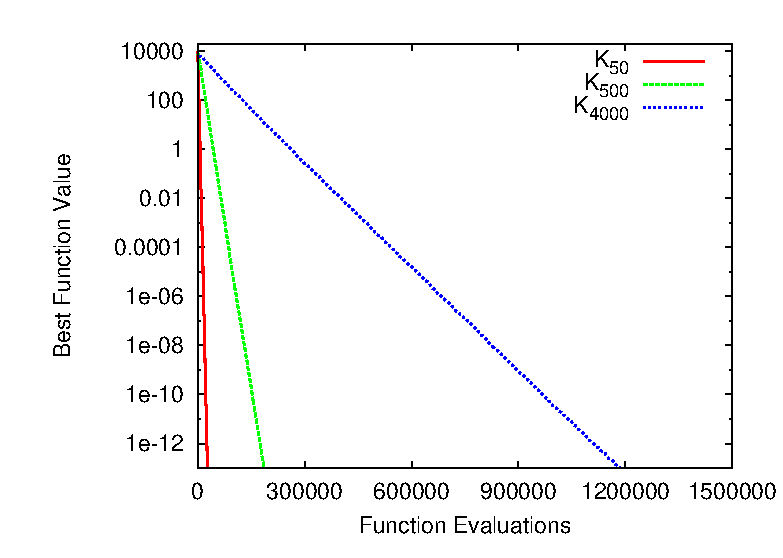
\includegraphics[height=.23\linewidth]{evals_sphere}\\
	\end{tabular}

  }

%%%%%%%%%%%%%%%%%%%%%%%%%%%%%%%%%%%%%%%%%%%%%%%%%%%%%%%%%%%%%%%%%%%%%%%%%%%%%%
  \headerbox{Speculative Evaluation: Reproducing PSO two iterations at a time}
  {name=description,column=0,span=3,below=diminishing}{
%%%%%%%%%%%%%%%%%%%%%%%%%%%%%%%%%%%%%%%%%%%%%%%%%%%%%%%%%%%%%%%%%%%%%%%%%%%%%%

	\begin{tabular}{cc}
	  \ \ \ \ \ \ \ \ \ \ \ \ \ \ \ \ \ \ \ \ \ \ \ &
	  \includegraphics[height=.33\linewidth]{speculative_evaluation} \\
	\end{tabular}

	With some bookkeeping, we can figure out which evaluation to keep to
	exactly reproduce PSO, two iterations at a time.  See the paper for more
	details.

  }

%%%%%%%%%%%%%%%%%%%%%%%%%%%%%%%%%%%%%%%%%%%%%%%%%%%%%%%%%%%%%%%%%%%%%%%%%%%%%%
  \headerbox{Results}
  {name=results,column=0,span=3,below=description}{
%%%%%%%%%%%%%%%%%%%%%%%%%%%%%%%%%%%%%%%%%%%%%%%%%%%%%%%%%%%%%%%%%%%%%%%%%%%%%%

	\begin{tabular}{ccc}
	  \centering
	  Sphere&Griewank&Bohachevsky\\
	  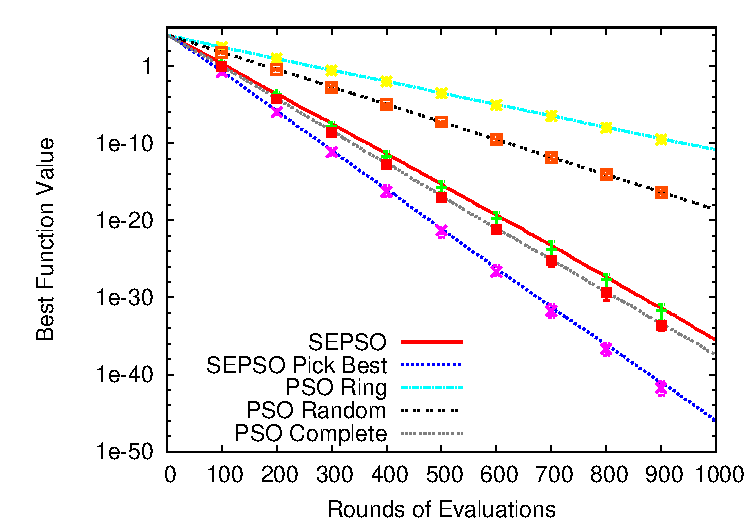
\includegraphics[height=.22\linewidth]{sphere}&
	  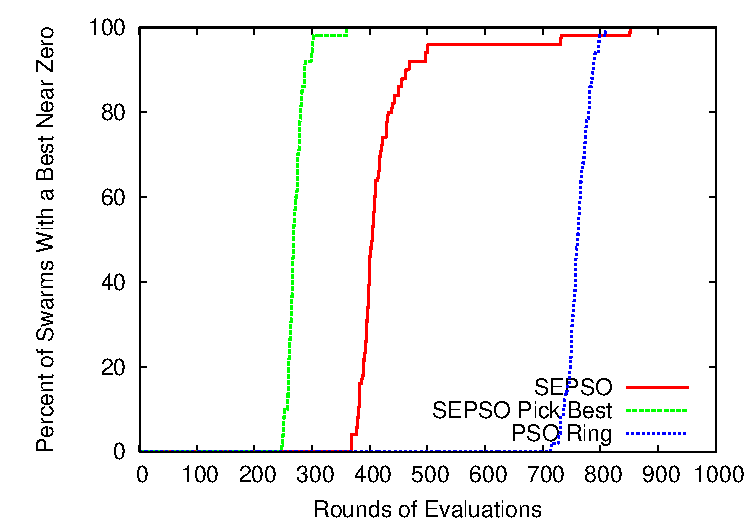
\includegraphics[height=.22\linewidth]{griewank}&
	  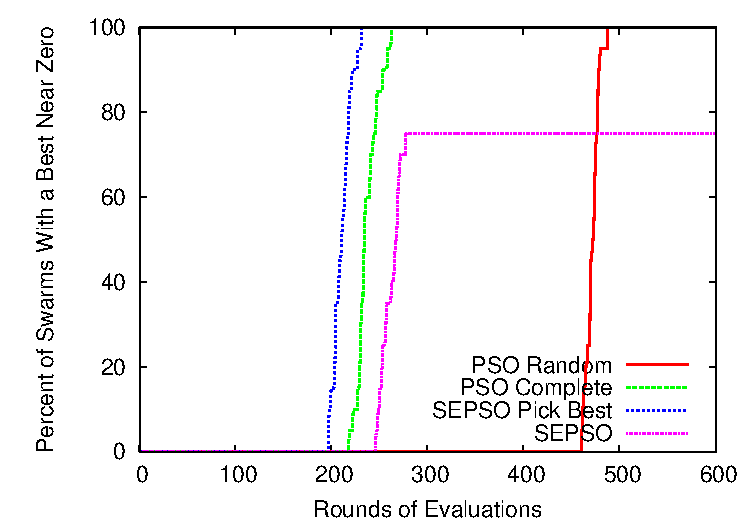
\includegraphics[height=.22\linewidth]{bohachevsky}\\
	\end{tabular}

  }

\end{poster}

\end{document}
